\documentclass[10pt]{article}
    \usepackage[utf8]{inputenc}
    \usepackage{amsmath}
    \usepackage[margin=0.5in]{geometry}
    \usepackage{graphicx}
    \usepackage{caption}
    \usepackage{subcaption}

    \title{Machine Learning Coursework 2}
    \author{Nashe Mncube:nm15042 David Sharp:ds16797}
    \date{November 2018}

    \begin{document}
    \maketitle

    \section{Question 5}
    Considering first $KL(p(\mathbf{x})||q(\mathbf{x}))$ when $p(\mathbf{x})$ is large and $q(\mathbf{x})$ is near zero
    the KL divergence is massive, whereas when $p(\mathbf{x})$ is near zero and $q(\mathbf{x})$ is large, i.e we've
    overestimated $p(\mathbf{x})$ this is far less of a problem resulting in a smaller KL divergence.
    It is better to overfit $p(\mathbf{x})$, and to cover the non-zero parts of $p(\mathbf{x})$ than it is
    to have near zero points of $q(\mathbf{x})$ where large points of $p(\mathbf{x})$ exist.
    Considering instead $KL(q(\mathbf{x})||p(\mathbf{x}))$ the reverse occurs. If our approximation is large when the
    original distribution is small then the KL divergence will be large and if the approximation is small while the
    original distribution is large then we don't care much and the KL divergence is small.

    \section{Question 6}

    \begin{figure}[h]
        \caption{Original Image, Gaussian and Pepper noise, denoised with Variational Bayes}
        \centering
        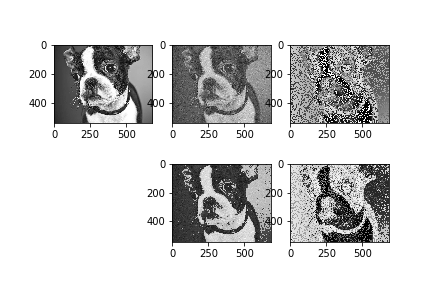
\includegraphics[width=0.5\textwidth]{/assets/vb/7iteration8neighbourGrey.png}
        \label{fig:variationalBayes}
    \end{figure}

    As before with Gibbs sampling we experimented with the number of iterations before the denoising results stopped
    getting any noticeably better. The Gaussian noise saw the greatest denoising effect with just a single iteration,
    due to the nature of the Gaussian noise.
    The Salt and Pepper noise however required a couple more iterations to stabilise, like with Gibbs and ICM, our particular
    image had inverted colours due to the noise. After around a dozen iterations as lot of random pixel noise was gone
    from the image and the original patterns on our pug are easily visible. Beyond around 25 iterations there are
    few further improvements in denoising.




  \end{document}
